\section{Wpływ skokowej zmiany sygnału zakłócenia}
\label{projekt:zad5}
-------POLECENIE--------

Załozyc, ze oprócz zmian sygnału wartosci zadanej nastepuje skokowa zmiana sygnału
zakłócenia z wartosci 0 do 1 (zmiana ta ma miejsce po osiagnieciu przez proces wartosci
zadanej wyjscia). Dobrac parametr Dz. Zamiescic wybrane wyniki symulacji. Pokazac,
ze pomiar zakłócenia i jego uwzglednienie prowadzi do lepszej regulacji niz gdy brak
jest tego pomiaru.

-------POLECENIE--------



\subsection{Dobór parametru $D_z$}
\label{projekt:zad5:Dz}

Parametr Dz jest to liczba próbek, dla której następuje stabilizacja odpowiedzi skokowych toru zakłóceń, 
dobrano go na podstawie analizy odpowiedzi skoku
zakłócenia z 0 na 1.
Dz wynosi = 75

\subsection{Regulacja bez uwzględnienia zakłócenia}
\label{projekt:zad5:regulacjaBezUwzg}

Po osiągnięciu przez proces wartości zadanej wyjścia następuje zmiana sygnału
zakłócenia z wartości 0 na 1.

\begin{figure}[H] 
    \centering
    % This file was created by matlab2tikz.
%
\definecolor{mycolor1}{rgb}{0.00000,0.44700,0.74100}%
\definecolor{mycolor2}{rgb}{0.85000,0.32500,0.09800}%
%
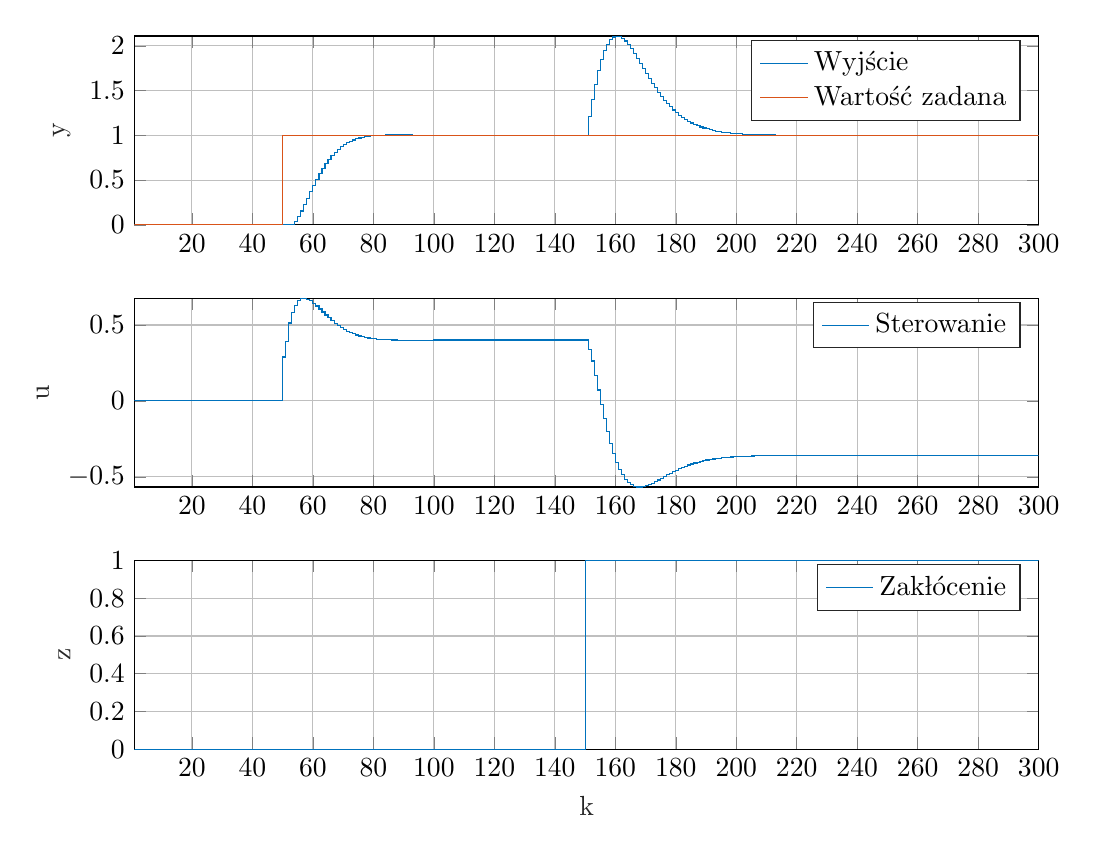
\begin{tikzpicture}

\begin{axis}[%
width=4.521in,
height=0.944in,
at={(0.758in,1.792in)},
scale only axis,
xmin=1,
xmax=300,
ymin=-0.56747,
ymax=0.67664,
ylabel style={font=\color{white!15!black}},
ylabel={u},
axis background/.style={fill=white},
xmajorgrids,
ymajorgrids,
legend style={legend cell align=left, align=left, draw=white!15!black}
]
\addplot[const plot, color=mycolor1] table[row sep=crcr] {%
1	0\\
2	0\\
3	0\\
4	0\\
5	0\\
6	0\\
7	0\\
8	0\\
9	0\\
10	0\\
11	0\\
12	0\\
13	0\\
14	0\\
15	0\\
16	0\\
17	0\\
18	0\\
19	0\\
20	0\\
21	0\\
22	0\\
23	0\\
24	0\\
25	0\\
26	0\\
27	0\\
28	0\\
29	0\\
30	0\\
31	0\\
32	0\\
33	0\\
34	0\\
35	0\\
36	0\\
37	0\\
38	0\\
39	0\\
40	0\\
41	0\\
42	0\\
43	0\\
44	0\\
45	0\\
46	0\\
47	0\\
48	0\\
49	0\\
50	0.28956\\
51	0.39251\\
52	0.5131\\
53	0.58007\\
54	0.63135\\
55	0.65951\\
56	0.67407\\
57	0.67664\\
58	0.67103\\
59	0.65931\\
60	0.64358\\
61	0.62529\\
62	0.60567\\
63	0.58562\\
64	0.56581\\
65	0.54674\\
66	0.52873\\
67	0.512\\
68	0.49669\\
69	0.48283\\
70	0.47042\\
71	0.45942\\
72	0.44977\\
73	0.44136\\
74	0.4341\\
75	0.42788\\
76	0.4226\\
77	0.41815\\
78	0.41444\\
79	0.41136\\
80	0.40884\\
81	0.4068\\
82	0.40516\\
83	0.40387\\
84	0.40286\\
85	0.40209\\
86	0.40151\\
87	0.4011\\
88	0.40081\\
89	0.40063\\
90	0.40052\\
91	0.40048\\
92	0.40048\\
93	0.40051\\
94	0.40057\\
95	0.40065\\
96	0.40073\\
97	0.40082\\
98	0.40091\\
99	0.401\\
100	0.40108\\
101	0.40116\\
102	0.40123\\
103	0.4013\\
104	0.40136\\
105	0.40142\\
106	0.40146\\
107	0.4015\\
108	0.40154\\
109	0.40157\\
110	0.4016\\
111	0.40162\\
112	0.40164\\
113	0.40166\\
114	0.40167\\
115	0.40168\\
116	0.40169\\
117	0.4017\\
118	0.4017\\
119	0.40171\\
120	0.40171\\
121	0.40171\\
122	0.40171\\
123	0.40172\\
124	0.40172\\
125	0.40172\\
126	0.40172\\
127	0.40172\\
128	0.40172\\
129	0.40172\\
130	0.40172\\
131	0.40172\\
132	0.40172\\
133	0.40171\\
134	0.40171\\
135	0.40171\\
136	0.40171\\
137	0.40171\\
138	0.40171\\
139	0.40171\\
140	0.40171\\
141	0.40171\\
142	0.40171\\
143	0.40171\\
144	0.40171\\
145	0.40171\\
146	0.40171\\
147	0.40171\\
148	0.40171\\
149	0.40171\\
150	0.40171\\
151	0.33996\\
152	0.26319\\
153	0.16932\\
154	0.071704\\
155	-0.025885\\
156	-0.11852\\
157	-0.20385\\
158	-0.28015\\
159	-0.34667\\
160	-0.40322\\
161	-0.45005\\
162	-0.48772\\
163	-0.51696\\
164	-0.53862\\
165	-0.55362\\
166	-0.56285\\
167	-0.56719\\
168	-0.56747\\
169	-0.56444\\
170	-0.55878\\
171	-0.55109\\
172	-0.54192\\
173	-0.53171\\
174	-0.52084\\
175	-0.50963\\
176	-0.49835\\
177	-0.4872\\
178	-0.47635\\
179	-0.46592\\
180	-0.456\\
181	-0.44665\\
182	-0.43791\\
183	-0.4298\\
184	-0.42232\\
185	-0.41546\\
186	-0.4092\\
187	-0.40352\\
188	-0.39839\\
189	-0.39377\\
190	-0.38963\\
191	-0.38593\\
192	-0.38263\\
193	-0.37971\\
194	-0.37712\\
195	-0.37483\\
196	-0.37281\\
197	-0.37104\\
198	-0.36948\\
199	-0.36812\\
200	-0.36693\\
201	-0.36589\\
202	-0.36498\\
203	-0.36419\\
204	-0.3635\\
205	-0.3629\\
206	-0.36238\\
207	-0.36193\\
208	-0.36154\\
209	-0.3612\\
210	-0.36091\\
211	-0.36065\\
212	-0.36042\\
213	-0.36023\\
214	-0.36006\\
215	-0.35991\\
216	-0.35978\\
217	-0.35967\\
218	-0.35957\\
219	-0.35949\\
220	-0.35941\\
221	-0.35934\\
222	-0.35928\\
223	-0.35923\\
224	-0.35918\\
225	-0.35914\\
226	-0.35911\\
227	-0.35907\\
228	-0.35904\\
229	-0.35902\\
230	-0.35899\\
231	-0.35897\\
232	-0.35896\\
233	-0.35894\\
234	-0.35893\\
235	-0.35892\\
236	-0.35891\\
237	-0.3589\\
238	-0.3589\\
239	-0.35889\\
240	-0.35889\\
241	-0.35888\\
242	-0.35888\\
243	-0.35887\\
244	-0.35887\\
245	-0.35887\\
246	-0.35887\\
247	-0.35886\\
248	-0.35886\\
249	-0.35886\\
250	-0.35886\\
251	-0.35885\\
252	-0.35885\\
253	-0.35885\\
254	-0.35885\\
255	-0.35885\\
256	-0.35885\\
257	-0.35884\\
258	-0.35884\\
259	-0.35884\\
260	-0.35884\\
261	-0.35884\\
262	-0.35884\\
263	-0.35884\\
264	-0.35884\\
265	-0.35884\\
266	-0.35884\\
267	-0.35884\\
268	-0.35883\\
269	-0.35883\\
270	-0.35883\\
271	-0.35883\\
272	-0.35883\\
273	-0.35883\\
274	-0.35883\\
275	-0.35883\\
276	-0.35883\\
277	-0.35883\\
278	-0.35883\\
279	-0.35883\\
280	-0.35883\\
281	-0.35883\\
282	-0.35883\\
283	-0.35883\\
284	-0.35883\\
285	-0.35883\\
286	-0.35883\\
287	-0.35883\\
288	-0.35883\\
289	-0.35883\\
290	-0.35883\\
291	-0.35883\\
292	-0.35883\\
293	-0.35883\\
294	-0.35883\\
295	-0.35883\\
296	-0.35883\\
297	-0.35883\\
298	-0.35883\\
299	-0.35883\\
300	-0.35884\\
};
\addlegendentry{Sterowanie}

\end{axis}

\begin{axis}[%
width=4.521in,
height=0.944in,
at={(0.758in,3.103in)},
scale only axis,
xmin=1,
xmax=300,
ymin=0,
ymax=2.1093,
ylabel style={font=\color{white!15!black}},
ylabel={y},
axis background/.style={fill=white},
xmajorgrids,
ymajorgrids,
legend style={legend cell align=left, align=left, draw=white!15!black}
]
\addplot[const plot, color=mycolor1] table[row sep=crcr] {%
1	0\\
2	0\\
3	0\\
4	0\\
5	0\\
6	0\\
7	0\\
8	0\\
9	0\\
10	0\\
11	0\\
12	0\\
13	0\\
14	0\\
15	0\\
16	0\\
17	0\\
18	0\\
19	0\\
20	0\\
21	0\\
22	0\\
23	0\\
24	0\\
25	0\\
26	0\\
27	0\\
28	0\\
29	0\\
30	0\\
31	0\\
32	0\\
33	0\\
34	0\\
35	0\\
36	0\\
37	0\\
38	0\\
39	0\\
40	0\\
41	0\\
42	0\\
43	0\\
44	0\\
45	0\\
46	0\\
47	0\\
48	0\\
49	0\\
50	0\\
51	0\\
52	0\\
53	0\\
54	0.039119\\
55	0.090032\\
56	0.15448\\
57	0.22449\\
58	0.29764\\
59	0.37063\\
60	0.44164\\
61	0.50914\\
62	0.57223\\
63	0.63032\\
64	0.68313\\
65	0.73061\\
66	0.77286\\
67	0.81011\\
68	0.84266\\
69	0.87086\\
70	0.8951\\
71	0.91576\\
72	0.93322\\
73	0.94786\\
74	0.96003\\
75	0.97004\\
76	0.97821\\
77	0.98479\\
78	0.99003\\
79	0.99414\\
80	0.99731\\
81	0.99971\\
82	1.0015\\
83	1.0027\\
84	1.0036\\
85	1.0041\\
86	1.0043\\
87	1.0044\\
88	1.0043\\
89	1.0042\\
90	1.0039\\
91	1.0036\\
92	1.0033\\
93	1.003\\
94	1.0027\\
95	1.0024\\
96	1.0021\\
97	1.0018\\
98	1.0016\\
99	1.0013\\
100	1.0011\\
101	1.001\\
102	1.0008\\
103	1.0007\\
104	1.0005\\
105	1.0004\\
106	1.0003\\
107	1.0003\\
108	1.0002\\
109	1.0002\\
110	1.0001\\
111	1.0001\\
112	1.0001\\
113	1\\
114	1\\
115	1\\
116	1\\
117	0.99999\\
118	0.99998\\
119	0.99998\\
120	0.99998\\
121	0.99998\\
122	0.99998\\
123	0.99998\\
124	0.99998\\
125	0.99998\\
126	0.99998\\
127	0.99998\\
128	0.99998\\
129	0.99998\\
130	0.99998\\
131	0.99998\\
132	0.99999\\
133	0.99999\\
134	0.99999\\
135	0.99999\\
136	0.99999\\
137	0.99999\\
138	0.99999\\
139	0.99999\\
140	0.99999\\
141	0.99999\\
142	0.99999\\
143	0.99999\\
144	0.99999\\
145	0.99999\\
146	0.99999\\
147	0.99999\\
148	0.99999\\
149	0.99999\\
150	0.99999\\
151	1.2132\\
152	1.4026\\
153	1.5706\\
154	1.7198\\
155	1.8439\\
156	1.9432\\
157	2.0176\\
158	2.0687\\
159	2.0984\\
160	2.1093\\
161	2.1037\\
162	2.0844\\
163	2.0537\\
164	2.0141\\
165	1.9677\\
166	1.9163\\
167	1.8617\\
168	1.8053\\
169	1.7482\\
170	1.6915\\
171	1.6361\\
172	1.5824\\
173	1.531\\
174	1.4823\\
175	1.4365\\
176	1.3936\\
177	1.3539\\
178	1.3172\\
179	1.2835\\
180	1.2527\\
181	1.2247\\
182	1.1993\\
183	1.1764\\
184	1.1559\\
185	1.1374\\
186	1.121\\
187	1.1063\\
188	1.0932\\
189	1.0817\\
190	1.0715\\
191	1.0625\\
192	1.0546\\
193	1.0476\\
194	1.0415\\
195	1.0361\\
196	1.0314\\
197	1.0274\\
198	1.0238\\
199	1.0207\\
200	1.018\\
201	1.0156\\
202	1.0136\\
203	1.0118\\
204	1.0103\\
205	1.0089\\
206	1.0078\\
207	1.0067\\
208	1.0059\\
209	1.0051\\
210	1.0044\\
211	1.0039\\
212	1.0034\\
213	1.0029\\
214	1.0025\\
215	1.0022\\
216	1.0019\\
217	1.0017\\
218	1.0014\\
219	1.0013\\
220	1.0011\\
221	1.0009\\
222	1.0008\\
223	1.0007\\
224	1.0006\\
225	1.0005\\
226	1.0004\\
227	1.0004\\
228	1.0003\\
229	1.0003\\
230	1.0002\\
231	1.0002\\
232	1.0002\\
233	1.0001\\
234	1.0001\\
235	1.0001\\
236	1.0001\\
237	1.0001\\
238	1\\
239	1\\
240	1\\
241	1\\
242	1\\
243	1\\
244	1\\
245	1\\
246	0.99999\\
247	0.99999\\
248	0.99999\\
249	0.99998\\
250	0.99998\\
251	0.99998\\
252	0.99998\\
253	0.99998\\
254	0.99998\\
255	0.99998\\
256	0.99998\\
257	0.99998\\
258	0.99998\\
259	0.99998\\
260	0.99998\\
261	0.99998\\
262	0.99998\\
263	0.99998\\
264	0.99998\\
265	0.99998\\
266	0.99998\\
267	0.99998\\
268	0.99999\\
269	0.99999\\
270	0.99999\\
271	0.99999\\
272	0.99999\\
273	0.99999\\
274	0.99999\\
275	0.99999\\
276	1\\
277	1\\
278	1\\
279	1\\
280	1\\
281	1\\
282	1\\
283	1\\
284	1\\
285	1\\
286	1\\
287	1\\
288	1\\
289	1\\
290	1\\
291	1\\
292	1\\
293	1\\
294	1\\
295	1\\
296	1\\
297	1\\
298	1\\
299	1\\
300	1\\
};
\addlegendentry{Wyjście}

\addplot[const plot, color=mycolor2] table[row sep=crcr] {%
1	0\\
2	0\\
3	0\\
4	0\\
5	0\\
6	0\\
7	0\\
8	0\\
9	0\\
10	0\\
11	0\\
12	0\\
13	0\\
14	0\\
15	0\\
16	0\\
17	0\\
18	0\\
19	0\\
20	0\\
21	0\\
22	0\\
23	0\\
24	0\\
25	0\\
26	0\\
27	0\\
28	0\\
29	0\\
30	0\\
31	0\\
32	0\\
33	0\\
34	0\\
35	0\\
36	0\\
37	0\\
38	0\\
39	0\\
40	0\\
41	0\\
42	0\\
43	0\\
44	0\\
45	0\\
46	0\\
47	0\\
48	0\\
49	0\\
50	1\\
51	1\\
52	1\\
53	1\\
54	1\\
55	1\\
56	1\\
57	1\\
58	1\\
59	1\\
60	1\\
61	1\\
62	1\\
63	1\\
64	1\\
65	1\\
66	1\\
67	1\\
68	1\\
69	1\\
70	1\\
71	1\\
72	1\\
73	1\\
74	1\\
75	1\\
76	1\\
77	1\\
78	1\\
79	1\\
80	1\\
81	1\\
82	1\\
83	1\\
84	1\\
85	1\\
86	1\\
87	1\\
88	1\\
89	1\\
90	1\\
91	1\\
92	1\\
93	1\\
94	1\\
95	1\\
96	1\\
97	1\\
98	1\\
99	1\\
100	1\\
101	1\\
102	1\\
103	1\\
104	1\\
105	1\\
106	1\\
107	1\\
108	1\\
109	1\\
110	1\\
111	1\\
112	1\\
113	1\\
114	1\\
115	1\\
116	1\\
117	1\\
118	1\\
119	1\\
120	1\\
121	1\\
122	1\\
123	1\\
124	1\\
125	1\\
126	1\\
127	1\\
128	1\\
129	1\\
130	1\\
131	1\\
132	1\\
133	1\\
134	1\\
135	1\\
136	1\\
137	1\\
138	1\\
139	1\\
140	1\\
141	1\\
142	1\\
143	1\\
144	1\\
145	1\\
146	1\\
147	1\\
148	1\\
149	1\\
150	1\\
151	1\\
152	1\\
153	1\\
154	1\\
155	1\\
156	1\\
157	1\\
158	1\\
159	1\\
160	1\\
161	1\\
162	1\\
163	1\\
164	1\\
165	1\\
166	1\\
167	1\\
168	1\\
169	1\\
170	1\\
171	1\\
172	1\\
173	1\\
174	1\\
175	1\\
176	1\\
177	1\\
178	1\\
179	1\\
180	1\\
181	1\\
182	1\\
183	1\\
184	1\\
185	1\\
186	1\\
187	1\\
188	1\\
189	1\\
190	1\\
191	1\\
192	1\\
193	1\\
194	1\\
195	1\\
196	1\\
197	1\\
198	1\\
199	1\\
200	1\\
201	1\\
202	1\\
203	1\\
204	1\\
205	1\\
206	1\\
207	1\\
208	1\\
209	1\\
210	1\\
211	1\\
212	1\\
213	1\\
214	1\\
215	1\\
216	1\\
217	1\\
218	1\\
219	1\\
220	1\\
221	1\\
222	1\\
223	1\\
224	1\\
225	1\\
226	1\\
227	1\\
228	1\\
229	1\\
230	1\\
231	1\\
232	1\\
233	1\\
234	1\\
235	1\\
236	1\\
237	1\\
238	1\\
239	1\\
240	1\\
241	1\\
242	1\\
243	1\\
244	1\\
245	1\\
246	1\\
247	1\\
248	1\\
249	1\\
250	1\\
251	1\\
252	1\\
253	1\\
254	1\\
255	1\\
256	1\\
257	1\\
258	1\\
259	1\\
260	1\\
261	1\\
262	1\\
263	1\\
264	1\\
265	1\\
266	1\\
267	1\\
268	1\\
269	1\\
270	1\\
271	1\\
272	1\\
273	1\\
274	1\\
275	1\\
276	1\\
277	1\\
278	1\\
279	1\\
280	1\\
281	1\\
282	1\\
283	1\\
284	1\\
285	1\\
286	1\\
287	1\\
288	1\\
289	1\\
290	1\\
291	1\\
292	1\\
293	1\\
294	1\\
295	1\\
296	1\\
297	1\\
298	1\\
299	1\\
300	1\\
};
\addlegendentry{Wartość zadana}

\end{axis}

\begin{axis}[%
width=4.521in,
height=0.944in,
at={(0.758in,0.481in)},
scale only axis,
xmin=1,
xmax=300,
xlabel style={font=\color{white!15!black}},
xlabel={k},
ymin=0,
ymax=1,
ylabel style={font=\color{white!15!black}},
ylabel={z},
axis background/.style={fill=white},
xmajorgrids,
ymajorgrids,
legend style={legend cell align=left, align=left, draw=white!15!black}
]
\addplot[const plot, color=mycolor1] table[row sep=crcr] {%
1	0\\
2	0\\
3	0\\
4	0\\
5	0\\
6	0\\
7	0\\
8	0\\
9	0\\
10	0\\
11	0\\
12	0\\
13	0\\
14	0\\
15	0\\
16	0\\
17	0\\
18	0\\
19	0\\
20	0\\
21	0\\
22	0\\
23	0\\
24	0\\
25	0\\
26	0\\
27	0\\
28	0\\
29	0\\
30	0\\
31	0\\
32	0\\
33	0\\
34	0\\
35	0\\
36	0\\
37	0\\
38	0\\
39	0\\
40	0\\
41	0\\
42	0\\
43	0\\
44	0\\
45	0\\
46	0\\
47	0\\
48	0\\
49	0\\
50	0\\
51	0\\
52	0\\
53	0\\
54	0\\
55	0\\
56	0\\
57	0\\
58	0\\
59	0\\
60	0\\
61	0\\
62	0\\
63	0\\
64	0\\
65	0\\
66	0\\
67	0\\
68	0\\
69	0\\
70	0\\
71	0\\
72	0\\
73	0\\
74	0\\
75	0\\
76	0\\
77	0\\
78	0\\
79	0\\
80	0\\
81	0\\
82	0\\
83	0\\
84	0\\
85	0\\
86	0\\
87	0\\
88	0\\
89	0\\
90	0\\
91	0\\
92	0\\
93	0\\
94	0\\
95	0\\
96	0\\
97	0\\
98	0\\
99	0\\
100	0\\
101	0\\
102	0\\
103	0\\
104	0\\
105	0\\
106	0\\
107	0\\
108	0\\
109	0\\
110	0\\
111	0\\
112	0\\
113	0\\
114	0\\
115	0\\
116	0\\
117	0\\
118	0\\
119	0\\
120	0\\
121	0\\
122	0\\
123	0\\
124	0\\
125	0\\
126	0\\
127	0\\
128	0\\
129	0\\
130	0\\
131	0\\
132	0\\
133	0\\
134	0\\
135	0\\
136	0\\
137	0\\
138	0\\
139	0\\
140	0\\
141	0\\
142	0\\
143	0\\
144	0\\
145	0\\
146	0\\
147	0\\
148	0\\
149	0\\
150	1\\
151	1\\
152	1\\
153	1\\
154	1\\
155	1\\
156	1\\
157	1\\
158	1\\
159	1\\
160	1\\
161	1\\
162	1\\
163	1\\
164	1\\
165	1\\
166	1\\
167	1\\
168	1\\
169	1\\
170	1\\
171	1\\
172	1\\
173	1\\
174	1\\
175	1\\
176	1\\
177	1\\
178	1\\
179	1\\
180	1\\
181	1\\
182	1\\
183	1\\
184	1\\
185	1\\
186	1\\
187	1\\
188	1\\
189	1\\
190	1\\
191	1\\
192	1\\
193	1\\
194	1\\
195	1\\
196	1\\
197	1\\
198	1\\
199	1\\
200	1\\
201	1\\
202	1\\
203	1\\
204	1\\
205	1\\
206	1\\
207	1\\
208	1\\
209	1\\
210	1\\
211	1\\
212	1\\
213	1\\
214	1\\
215	1\\
216	1\\
217	1\\
218	1\\
219	1\\
220	1\\
221	1\\
222	1\\
223	1\\
224	1\\
225	1\\
226	1\\
227	1\\
228	1\\
229	1\\
230	1\\
231	1\\
232	1\\
233	1\\
234	1\\
235	1\\
236	1\\
237	1\\
238	1\\
239	1\\
240	1\\
241	1\\
242	1\\
243	1\\
244	1\\
245	1\\
246	1\\
247	1\\
248	1\\
249	1\\
250	1\\
251	1\\
252	1\\
253	1\\
254	1\\
255	1\\
256	1\\
257	1\\
258	1\\
259	1\\
260	1\\
261	1\\
262	1\\
263	1\\
264	1\\
265	1\\
266	1\\
267	1\\
268	1\\
269	1\\
270	1\\
271	1\\
272	1\\
273	1\\
274	1\\
275	1\\
276	1\\
277	1\\
278	1\\
279	1\\
280	1\\
281	1\\
282	1\\
283	1\\
284	1\\
285	1\\
286	1\\
287	1\\
288	1\\
289	1\\
290	1\\
291	1\\
292	1\\
293	1\\
294	1\\
295	1\\
296	1\\
297	1\\
298	1\\
299	1\\
300	1\\
};
\addlegendentry{Zakłócenie}

\end{axis}
\end{tikzpicture}%
    \caption{Regulacja bez uwzględnienia zakłócenia}
    \label{projekt:zad5:regulacjaBezUwzgZ:figure}
\end{figure}

\subsection{Regulacja z uwzględnieniem zakłócenia}
\label{projekt:zad5:regulacjaZUwzg}

Po osiągnięciu przez proces wartości zadanej wyjścia następuje zmiana sygnału
zakłócenia z wartości 0 na 1.

\begin{figure}[H] 
    \centering
    % This file was created by matlab2tikz.
%
\definecolor{mycolor1}{rgb}{0.00000,0.44700,0.74100}%
\definecolor{mycolor2}{rgb}{0.85000,0.32500,0.09800}%
%
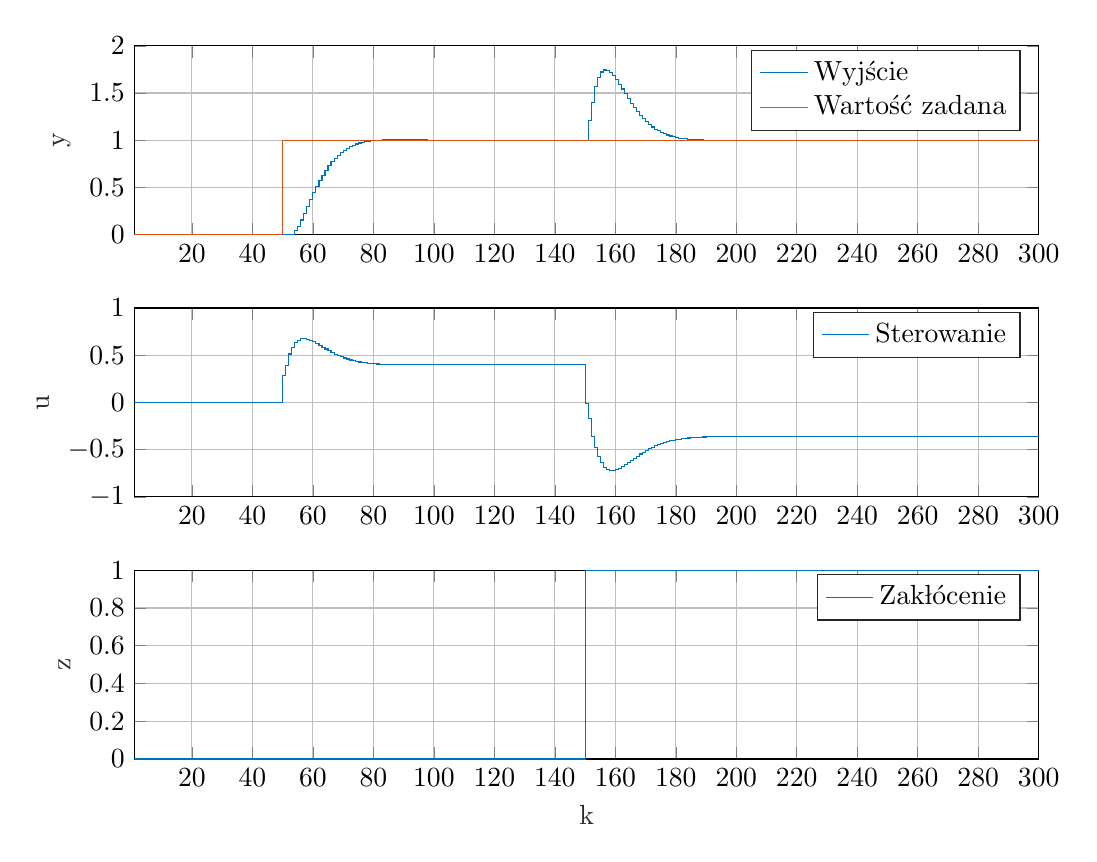
\begin{tikzpicture}

\begin{axis}[%
width=4.521in,
height=0.944in,
at={(0.758in,1.792in)},
scale only axis,
xmin=1,
xmax=300,
ymin=-1,
ymax=1,
ylabel style={font=\color{white!15!black}},
ylabel={u},
axis background/.style={fill=white},
xmajorgrids,
ymajorgrids,
legend style={legend cell align=left, align=left, draw=white!15!black}
]
\addplot[const plot, color=mycolor1] table[row sep=crcr] {%
1	0\\
2	0\\
3	0\\
4	0\\
5	0\\
6	0\\
7	0\\
8	0\\
9	0\\
10	0\\
11	0\\
12	0\\
13	0\\
14	0\\
15	0\\
16	0\\
17	0\\
18	0\\
19	0\\
20	0\\
21	0\\
22	0\\
23	0\\
24	0\\
25	0\\
26	0\\
27	0\\
28	0\\
29	0\\
30	0\\
31	0\\
32	0\\
33	0\\
34	0\\
35	0\\
36	0\\
37	0\\
38	0\\
39	0\\
40	0\\
41	0\\
42	0\\
43	0\\
44	0\\
45	0\\
46	0\\
47	0\\
48	0\\
49	0\\
50	0.28956\\
51	0.39251\\
52	0.5131\\
53	0.58007\\
54	0.63135\\
55	0.65951\\
56	0.67407\\
57	0.67664\\
58	0.67103\\
59	0.65931\\
60	0.64358\\
61	0.62529\\
62	0.60567\\
63	0.58562\\
64	0.56581\\
65	0.54674\\
66	0.52873\\
67	0.512\\
68	0.49669\\
69	0.48283\\
70	0.47042\\
71	0.45942\\
72	0.44977\\
73	0.44136\\
74	0.4341\\
75	0.42788\\
76	0.4226\\
77	0.41815\\
78	0.41444\\
79	0.41136\\
80	0.40884\\
81	0.4068\\
82	0.40516\\
83	0.40387\\
84	0.40286\\
85	0.40209\\
86	0.40151\\
87	0.4011\\
88	0.40081\\
89	0.40063\\
90	0.40052\\
91	0.40048\\
92	0.40048\\
93	0.40051\\
94	0.40057\\
95	0.40065\\
96	0.40073\\
97	0.40082\\
98	0.40091\\
99	0.401\\
100	0.40108\\
101	0.40116\\
102	0.40123\\
103	0.4013\\
104	0.40136\\
105	0.40142\\
106	0.40146\\
107	0.4015\\
108	0.40154\\
109	0.40157\\
110	0.4016\\
111	0.40162\\
112	0.40164\\
113	0.40166\\
114	0.40167\\
115	0.40168\\
116	0.40169\\
117	0.4017\\
118	0.4017\\
119	0.40171\\
120	0.40171\\
121	0.40171\\
122	0.40171\\
123	0.40172\\
124	0.40172\\
125	0.40172\\
126	0.40172\\
127	0.40172\\
128	0.40172\\
129	0.40172\\
130	0.40172\\
131	0.40172\\
132	0.40172\\
133	0.40171\\
134	0.40171\\
135	0.40171\\
136	0.40171\\
137	0.40171\\
138	0.40171\\
139	0.40171\\
140	0.40171\\
141	0.40171\\
142	0.40171\\
143	0.40171\\
144	0.40171\\
145	0.40171\\
146	0.40171\\
147	0.40171\\
148	0.40171\\
149	0.40171\\
150	-0.0084381\\
151	-0.16993\\
152	-0.3602\\
153	-0.47885\\
154	-0.57623\\
155	-0.64083\\
156	-0.68492\\
157	-0.71015\\
158	-0.7215\\
159	-0.72172\\
160	-0.71371\\
161	-0.69963\\
162	-0.68133\\
163	-0.66028\\
164	-0.63766\\
165	-0.61438\\
166	-0.59115\\
167	-0.56851\\
168	-0.54683\\
169	-0.52638\\
170	-0.50732\\
171	-0.48975\\
172	-0.47371\\
173	-0.45917\\
174	-0.44609\\
175	-0.43441\\
176	-0.42404\\
177	-0.41488\\
178	-0.40685\\
179	-0.39983\\
180	-0.39372\\
181	-0.38844\\
182	-0.38389\\
183	-0.37998\\
184	-0.37665\\
185	-0.3738\\
186	-0.37139\\
187	-0.36935\\
188	-0.36764\\
189	-0.3662\\
190	-0.36499\\
191	-0.36398\\
192	-0.36315\\
193	-0.36245\\
194	-0.36187\\
195	-0.36139\\
196	-0.361\\
197	-0.36067\\
198	-0.3604\\
199	-0.36018\\
200	-0.35999\\
201	-0.35984\\
202	-0.35971\\
203	-0.35961\\
204	-0.35952\\
205	-0.35944\\
206	-0.35937\\
207	-0.35932\\
208	-0.35927\\
209	-0.35923\\
210	-0.35919\\
211	-0.35915\\
212	-0.35912\\
213	-0.3591\\
214	-0.35907\\
215	-0.35905\\
216	-0.35903\\
217	-0.35901\\
218	-0.35899\\
219	-0.35897\\
220	-0.35896\\
221	-0.35894\\
222	-0.35893\\
223	-0.35892\\
224	-0.35891\\
225	-0.3589\\
226	-0.3589\\
227	-0.35889\\
228	-0.35889\\
229	-0.35889\\
230	-0.35889\\
231	-0.35889\\
232	-0.35888\\
233	-0.35888\\
234	-0.35888\\
235	-0.35888\\
236	-0.35888\\
237	-0.35888\\
238	-0.35888\\
239	-0.35888\\
240	-0.35888\\
241	-0.35888\\
242	-0.35887\\
243	-0.35887\\
244	-0.35887\\
245	-0.35887\\
246	-0.35887\\
247	-0.35886\\
248	-0.35886\\
249	-0.35886\\
250	-0.35886\\
251	-0.35886\\
252	-0.35885\\
253	-0.35885\\
254	-0.35885\\
255	-0.35885\\
256	-0.35885\\
257	-0.35885\\
258	-0.35884\\
259	-0.35884\\
260	-0.35884\\
261	-0.35884\\
262	-0.35884\\
263	-0.35884\\
264	-0.35884\\
265	-0.35884\\
266	-0.35884\\
267	-0.35884\\
268	-0.35883\\
269	-0.35883\\
270	-0.35883\\
271	-0.35883\\
272	-0.35883\\
273	-0.35883\\
274	-0.35883\\
275	-0.35883\\
276	-0.35883\\
277	-0.35883\\
278	-0.35883\\
279	-0.35883\\
280	-0.35883\\
281	-0.35883\\
282	-0.35883\\
283	-0.35883\\
284	-0.35883\\
285	-0.35883\\
286	-0.35883\\
287	-0.35883\\
288	-0.35883\\
289	-0.35883\\
290	-0.35883\\
291	-0.35883\\
292	-0.35883\\
293	-0.35883\\
294	-0.35884\\
295	-0.35884\\
296	-0.35884\\
297	-0.35884\\
298	-0.35884\\
299	-0.35884\\
300	-0.35884\\
};
\addlegendentry{Sterowanie}

\end{axis}

\begin{axis}[%
width=4.521in,
height=0.944in,
at={(0.758in,3.103in)},
scale only axis,
xmin=1,
xmax=300,
ymin=0,
ymax=2,
ylabel style={font=\color{white!15!black}},
ylabel={y},
axis background/.style={fill=white},
xmajorgrids,
ymajorgrids,
legend style={legend cell align=left, align=left, draw=white!15!black}
]
\addplot[const plot, color=mycolor1] table[row sep=crcr] {%
1	0\\
2	0\\
3	0\\
4	0\\
5	0\\
6	0\\
7	0\\
8	0\\
9	0\\
10	0\\
11	0\\
12	0\\
13	0\\
14	0\\
15	0\\
16	0\\
17	0\\
18	0\\
19	0\\
20	0\\
21	0\\
22	0\\
23	0\\
24	0\\
25	0\\
26	0\\
27	0\\
28	0\\
29	0\\
30	0\\
31	0\\
32	0\\
33	0\\
34	0\\
35	0\\
36	0\\
37	0\\
38	0\\
39	0\\
40	0\\
41	0\\
42	0\\
43	0\\
44	0\\
45	0\\
46	0\\
47	0\\
48	0\\
49	0\\
50	0\\
51	0\\
52	0\\
53	0\\
54	0.039119\\
55	0.090032\\
56	0.15448\\
57	0.22449\\
58	0.29764\\
59	0.37063\\
60	0.44164\\
61	0.50914\\
62	0.57223\\
63	0.63032\\
64	0.68313\\
65	0.73061\\
66	0.77286\\
67	0.81011\\
68	0.84266\\
69	0.87086\\
70	0.8951\\
71	0.91576\\
72	0.93322\\
73	0.94786\\
74	0.96003\\
75	0.97004\\
76	0.97821\\
77	0.98479\\
78	0.99003\\
79	0.99414\\
80	0.99731\\
81	0.99971\\
82	1.0015\\
83	1.0027\\
84	1.0036\\
85	1.0041\\
86	1.0043\\
87	1.0044\\
88	1.0043\\
89	1.0042\\
90	1.0039\\
91	1.0036\\
92	1.0033\\
93	1.003\\
94	1.0027\\
95	1.0024\\
96	1.0021\\
97	1.0018\\
98	1.0016\\
99	1.0013\\
100	1.0011\\
101	1.001\\
102	1.0008\\
103	1.0007\\
104	1.0005\\
105	1.0004\\
106	1.0003\\
107	1.0003\\
108	1.0002\\
109	1.0002\\
110	1.0001\\
111	1.0001\\
112	1.0001\\
113	1\\
114	1\\
115	1\\
116	1\\
117	0.99999\\
118	0.99998\\
119	0.99998\\
120	0.99998\\
121	0.99998\\
122	0.99998\\
123	0.99998\\
124	0.99998\\
125	0.99998\\
126	0.99998\\
127	0.99998\\
128	0.99998\\
129	0.99998\\
130	0.99998\\
131	0.99998\\
132	0.99999\\
133	0.99999\\
134	0.99999\\
135	0.99999\\
136	0.99999\\
137	0.99999\\
138	0.99999\\
139	0.99999\\
140	0.99999\\
141	0.99999\\
142	0.99999\\
143	0.99999\\
144	0.99999\\
145	0.99999\\
146	0.99999\\
147	0.99999\\
148	0.99999\\
149	0.99999\\
150	0.99999\\
151	1.2132\\
152	1.4026\\
153	1.5706\\
154	1.6644\\
155	1.7226\\
156	1.7442\\
157	1.7418\\
158	1.7203\\
159	1.6858\\
160	1.6425\\
161	1.5938\\
162	1.5424\\
163	1.4905\\
164	1.4394\\
165	1.3904\\
166	1.3442\\
167	1.3012\\
168	1.2618\\
169	1.226\\
170	1.1938\\
171	1.1651\\
172	1.1398\\
173	1.1176\\
174	1.0983\\
175	1.0816\\
176	1.0672\\
177	1.055\\
178	1.0446\\
179	1.0359\\
180	1.0286\\
181	1.0226\\
182	1.0176\\
183	1.0135\\
184	1.0103\\
185	1.0076\\
186	1.0055\\
187	1.0039\\
188	1.0026\\
189	1.0016\\
190	1.0009\\
191	1.0003\\
192	0.99996\\
193	0.99971\\
194	0.99955\\
195	0.99946\\
196	0.99942\\
197	0.99942\\
198	0.99945\\
199	0.99949\\
200	0.99955\\
201	0.99961\\
202	0.99967\\
203	0.99973\\
204	0.99979\\
205	0.99984\\
206	0.99989\\
207	0.99993\\
208	0.99997\\
209	1\\
210	1\\
211	1\\
212	1.0001\\
213	1.0001\\
214	1.0001\\
215	1.0001\\
216	1.0001\\
217	1.0001\\
218	1.0001\\
219	1.0001\\
220	1.0001\\
221	1.0001\\
222	1.0001\\
223	1.0001\\
224	1.0001\\
225	1.0001\\
226	1.0001\\
227	1.0001\\
228	1.0001\\
229	1.0001\\
230	1.0001\\
231	1.0001\\
232	1.0001\\
233	1.0001\\
234	1.0001\\
235	1.0001\\
236	1\\
237	1\\
238	1\\
239	1\\
240	1\\
241	1\\
242	1\\
243	1\\
244	1\\
245	1\\
246	1\\
247	1\\
248	1\\
249	0.99999\\
250	0.99999\\
251	0.99999\\
252	0.99999\\
253	0.99998\\
254	0.99998\\
255	0.99998\\
256	0.99998\\
257	0.99998\\
258	0.99998\\
259	0.99998\\
260	0.99998\\
261	0.99998\\
262	0.99998\\
263	0.99998\\
264	0.99998\\
265	0.99998\\
266	0.99999\\
267	0.99999\\
268	0.99999\\
269	0.99999\\
270	0.99999\\
271	0.99999\\
272	0.99999\\
273	0.99999\\
274	0.99999\\
275	1\\
276	1\\
277	1\\
278	1\\
279	1\\
280	1\\
281	1\\
282	1\\
283	1\\
284	1\\
285	1\\
286	1\\
287	1\\
288	1\\
289	1\\
290	1\\
291	1\\
292	1\\
293	1\\
294	1\\
295	1\\
296	1\\
297	1\\
298	1\\
299	1\\
300	1\\
};
\addlegendentry{Wyjście}

\addplot[const plot, color=mycolor2] table[row sep=crcr] {%
1	0\\
2	0\\
3	0\\
4	0\\
5	0\\
6	0\\
7	0\\
8	0\\
9	0\\
10	0\\
11	0\\
12	0\\
13	0\\
14	0\\
15	0\\
16	0\\
17	0\\
18	0\\
19	0\\
20	0\\
21	0\\
22	0\\
23	0\\
24	0\\
25	0\\
26	0\\
27	0\\
28	0\\
29	0\\
30	0\\
31	0\\
32	0\\
33	0\\
34	0\\
35	0\\
36	0\\
37	0\\
38	0\\
39	0\\
40	0\\
41	0\\
42	0\\
43	0\\
44	0\\
45	0\\
46	0\\
47	0\\
48	0\\
49	0\\
50	1\\
51	1\\
52	1\\
53	1\\
54	1\\
55	1\\
56	1\\
57	1\\
58	1\\
59	1\\
60	1\\
61	1\\
62	1\\
63	1\\
64	1\\
65	1\\
66	1\\
67	1\\
68	1\\
69	1\\
70	1\\
71	1\\
72	1\\
73	1\\
74	1\\
75	1\\
76	1\\
77	1\\
78	1\\
79	1\\
80	1\\
81	1\\
82	1\\
83	1\\
84	1\\
85	1\\
86	1\\
87	1\\
88	1\\
89	1\\
90	1\\
91	1\\
92	1\\
93	1\\
94	1\\
95	1\\
96	1\\
97	1\\
98	1\\
99	1\\
100	1\\
101	1\\
102	1\\
103	1\\
104	1\\
105	1\\
106	1\\
107	1\\
108	1\\
109	1\\
110	1\\
111	1\\
112	1\\
113	1\\
114	1\\
115	1\\
116	1\\
117	1\\
118	1\\
119	1\\
120	1\\
121	1\\
122	1\\
123	1\\
124	1\\
125	1\\
126	1\\
127	1\\
128	1\\
129	1\\
130	1\\
131	1\\
132	1\\
133	1\\
134	1\\
135	1\\
136	1\\
137	1\\
138	1\\
139	1\\
140	1\\
141	1\\
142	1\\
143	1\\
144	1\\
145	1\\
146	1\\
147	1\\
148	1\\
149	1\\
150	1\\
151	1\\
152	1\\
153	1\\
154	1\\
155	1\\
156	1\\
157	1\\
158	1\\
159	1\\
160	1\\
161	1\\
162	1\\
163	1\\
164	1\\
165	1\\
166	1\\
167	1\\
168	1\\
169	1\\
170	1\\
171	1\\
172	1\\
173	1\\
174	1\\
175	1\\
176	1\\
177	1\\
178	1\\
179	1\\
180	1\\
181	1\\
182	1\\
183	1\\
184	1\\
185	1\\
186	1\\
187	1\\
188	1\\
189	1\\
190	1\\
191	1\\
192	1\\
193	1\\
194	1\\
195	1\\
196	1\\
197	1\\
198	1\\
199	1\\
200	1\\
201	1\\
202	1\\
203	1\\
204	1\\
205	1\\
206	1\\
207	1\\
208	1\\
209	1\\
210	1\\
211	1\\
212	1\\
213	1\\
214	1\\
215	1\\
216	1\\
217	1\\
218	1\\
219	1\\
220	1\\
221	1\\
222	1\\
223	1\\
224	1\\
225	1\\
226	1\\
227	1\\
228	1\\
229	1\\
230	1\\
231	1\\
232	1\\
233	1\\
234	1\\
235	1\\
236	1\\
237	1\\
238	1\\
239	1\\
240	1\\
241	1\\
242	1\\
243	1\\
244	1\\
245	1\\
246	1\\
247	1\\
248	1\\
249	1\\
250	1\\
251	1\\
252	1\\
253	1\\
254	1\\
255	1\\
256	1\\
257	1\\
258	1\\
259	1\\
260	1\\
261	1\\
262	1\\
263	1\\
264	1\\
265	1\\
266	1\\
267	1\\
268	1\\
269	1\\
270	1\\
271	1\\
272	1\\
273	1\\
274	1\\
275	1\\
276	1\\
277	1\\
278	1\\
279	1\\
280	1\\
281	1\\
282	1\\
283	1\\
284	1\\
285	1\\
286	1\\
287	1\\
288	1\\
289	1\\
290	1\\
291	1\\
292	1\\
293	1\\
294	1\\
295	1\\
296	1\\
297	1\\
298	1\\
299	1\\
300	1\\
};
\addlegendentry{Wartość zadana}

\end{axis}

\begin{axis}[%
width=4.521in,
height=0.944in,
at={(0.758in,0.481in)},
scale only axis,
xmin=1,
xmax=300,
xlabel style={font=\color{white!15!black}},
xlabel={k},
ymin=0,
ymax=1,
ylabel style={font=\color{white!15!black}},
ylabel={z},
axis background/.style={fill=white},
xmajorgrids,
ymajorgrids,
legend style={legend cell align=left, align=left, draw=white!15!black}
]
\addplot[const plot, color=mycolor1] table[row sep=crcr] {%
1	0\\
2	0\\
3	0\\
4	0\\
5	0\\
6	0\\
7	0\\
8	0\\
9	0\\
10	0\\
11	0\\
12	0\\
13	0\\
14	0\\
15	0\\
16	0\\
17	0\\
18	0\\
19	0\\
20	0\\
21	0\\
22	0\\
23	0\\
24	0\\
25	0\\
26	0\\
27	0\\
28	0\\
29	0\\
30	0\\
31	0\\
32	0\\
33	0\\
34	0\\
35	0\\
36	0\\
37	0\\
38	0\\
39	0\\
40	0\\
41	0\\
42	0\\
43	0\\
44	0\\
45	0\\
46	0\\
47	0\\
48	0\\
49	0\\
50	0\\
51	0\\
52	0\\
53	0\\
54	0\\
55	0\\
56	0\\
57	0\\
58	0\\
59	0\\
60	0\\
61	0\\
62	0\\
63	0\\
64	0\\
65	0\\
66	0\\
67	0\\
68	0\\
69	0\\
70	0\\
71	0\\
72	0\\
73	0\\
74	0\\
75	0\\
76	0\\
77	0\\
78	0\\
79	0\\
80	0\\
81	0\\
82	0\\
83	0\\
84	0\\
85	0\\
86	0\\
87	0\\
88	0\\
89	0\\
90	0\\
91	0\\
92	0\\
93	0\\
94	0\\
95	0\\
96	0\\
97	0\\
98	0\\
99	0\\
100	0\\
101	0\\
102	0\\
103	0\\
104	0\\
105	0\\
106	0\\
107	0\\
108	0\\
109	0\\
110	0\\
111	0\\
112	0\\
113	0\\
114	0\\
115	0\\
116	0\\
117	0\\
118	0\\
119	0\\
120	0\\
121	0\\
122	0\\
123	0\\
124	0\\
125	0\\
126	0\\
127	0\\
128	0\\
129	0\\
130	0\\
131	0\\
132	0\\
133	0\\
134	0\\
135	0\\
136	0\\
137	0\\
138	0\\
139	0\\
140	0\\
141	0\\
142	0\\
143	0\\
144	0\\
145	0\\
146	0\\
147	0\\
148	0\\
149	0\\
150	1\\
151	1\\
152	1\\
153	1\\
154	1\\
155	1\\
156	1\\
157	1\\
158	1\\
159	1\\
160	1\\
161	1\\
162	1\\
163	1\\
164	1\\
165	1\\
166	1\\
167	1\\
168	1\\
169	1\\
170	1\\
171	1\\
172	1\\
173	1\\
174	1\\
175	1\\
176	1\\
177	1\\
178	1\\
179	1\\
180	1\\
181	1\\
182	1\\
183	1\\
184	1\\
185	1\\
186	1\\
187	1\\
188	1\\
189	1\\
190	1\\
191	1\\
192	1\\
193	1\\
194	1\\
195	1\\
196	1\\
197	1\\
198	1\\
199	1\\
200	1\\
201	1\\
202	1\\
203	1\\
204	1\\
205	1\\
206	1\\
207	1\\
208	1\\
209	1\\
210	1\\
211	1\\
212	1\\
213	1\\
214	1\\
215	1\\
216	1\\
217	1\\
218	1\\
219	1\\
220	1\\
221	1\\
222	1\\
223	1\\
224	1\\
225	1\\
226	1\\
227	1\\
228	1\\
229	1\\
230	1\\
231	1\\
232	1\\
233	1\\
234	1\\
235	1\\
236	1\\
237	1\\
238	1\\
239	1\\
240	1\\
241	1\\
242	1\\
243	1\\
244	1\\
245	1\\
246	1\\
247	1\\
248	1\\
249	1\\
250	1\\
251	1\\
252	1\\
253	1\\
254	1\\
255	1\\
256	1\\
257	1\\
258	1\\
259	1\\
260	1\\
261	1\\
262	1\\
263	1\\
264	1\\
265	1\\
266	1\\
267	1\\
268	1\\
269	1\\
270	1\\
271	1\\
272	1\\
273	1\\
274	1\\
275	1\\
276	1\\
277	1\\
278	1\\
279	1\\
280	1\\
281	1\\
282	1\\
283	1\\
284	1\\
285	1\\
286	1\\
287	1\\
288	1\\
289	1\\
290	1\\
291	1\\
292	1\\
293	1\\
294	1\\
295	1\\
296	1\\
297	1\\
298	1\\
299	1\\
300	1\\
};
\addlegendentry{Zakłócenie}

\end{axis}
\end{tikzpicture}%
    \caption{Regulacja z uwzględnieniem zakłócenia}
    \label{projekt:zad5:regulacjaUwzgZ:figure}
\end{figure}

\subsection{Porównanie wskaźnika jakości}
\label{projekt:zad5:porownanie}

Dla symulacji regulowanego obiektu bez pomiaru zakłóceń wynosi on:

Dla symulacji regulowanego obiektu z pomiarem zakłóceń wynosi on:

Wnioski: 

Uwzględnienie mierzalnego zakłócenia w algorytmie regulacji jest bardzo dobrym rozwiązaniem, 
odsprzęganie zakłócenia powoduje kompensację uchybu regulacji, 
a co za tym idzie wskaźnik jakości jest lepszy, 
a sama regulacja uznana jest za lepszą.

